
\chapter{Implementación} 


Debido a que nos encontramos en un terreno carente de fundamentos teóricos, nuestra mejor arma para probar que grado de aproximación de los problemas inversos son consistentes es por medio de experimentación metodológica. Esto nos permite revelar obstáculos del nuevo método así como también las grandes ventajas. 

Gran parte del trabajo de tesis se centra primordialmente en la experimentación con la propuesta innovadora para la solución bayesiana del problema inverso. Se hacen los experimentos con una implementación en Python cuyo código se encuentra adjunto. 


\section{Modelos de trabajo}

Existen una variedad de modelos a los que se puede aplicar la metodología descrita para problemas inversos. De hecho se puede implementar para cualquier modelo descrito por una ecuación diferencial ordinaria. Sin embargo, cada modelo tiene sus bemoles, lo que dificulta calibrar (en general), para cada aspecto en la distribución de los parámetros, como puede ser el caso de tomar las distribuciones a priori adecuadas, la variación de la muestra, los dominios adecuados para graficar las distribuciones a posterior, entre otras. Por ello, nos permitiremos enfocarnos en solo un par de modelos que son el modelo gravitatorio sujeto a fricción para un partícula en caída y el modelo de crecimiento logístico para una población en crecimiento. 


\subsection{Modelo Gravitatorio}

Consideremos una partícula puntual en un campo gravitatorio cercano a la superficie terrestre. Por medio de la dinámica clásica podemos modelar dicha caída con las leyes de Newton. Sea $x(t)$ la distancia recorrida (unidimensional) por la partícula puntual en el tiempo $t$. De la segunda ley de Newton sabemos que
\begin{align}
    \sum F_i = m\ddot{x}(t) 
    \label{3.1.01}
\end{align}
donde $\sum F_i$ es la suma de fuerzas ejercida sobre la partícula con masa $m$. 

Para el modelo de caída libre nos dice que la fuerza ejercida en la partícula es constante y se le conoce como constante de aceleración gravitacional $g$. De forma que la trayectoria se rige de (\ref{3.1.01}) con únicamente la fuerza gravitacional $F = mg$. La ecuación de la dinámica es 
\begin{align*}
    \ddot{x}(t) = g
\end{align*}
bajo las condiciones iniciales $x(0) = x_0, \dot{x}(0) = v_0$. La solución a la ecuación dinámica es \cite{sears1986fisica}
\begin{align*}
    x(t) = \frac{1}{2}gt^2 + v_0 t + x_0
\end{align*}

Sin embargo, dentro del marco establecido para el modelo gravitacional, no es un modelo realista ya que este no está considerando la desaceleración producto de la fricción con el medio que interactúa (aire). Por ello es necesario modelar la fuerza de fricción de forma adecuada. Un modelo físico plausible para la fricción es considerar una fuerza opuesta a la fuerza de gravedad y que está depende de la velocidad de la partícula. Consideremos dicha fuerza de fricción como $F_f = -bv(x) $. Podemos pensar que el modelo para la fuerza de fricción es una aproximación de los primeros polinomios de Taylor a primer grado, donde se descarta el termino constante ya que no tiene sentido físico que la fricción obedezca a marcos de referencia. 

El modelo que estamos interesados es entonces el \textbf{modelo gravitatorio sujeto a fricción}, cuya ecuación dinámica es 
\begin{align}
    m \ddot{x} = mg - b\dot{x}
    \label{3.1.03}
\end{align}
que representa la trayectoria de la partícula sujeta a dos fuerzas opuestas, la gravitatoria y la fricción con el medio. Además con las condiciones iniciales $x(0) = x_0, \dot{x}(0) = v_0$ Notemos que dados los parámetros $\theta = (g,b)$ podemos determinar unívocamente la trayectoria de interés. 

Para poder hacer inferencia bayesiana en el problema inverso, es necesario construir el forward map $F(\theta)$. Esto puede ser de dos maneras, podemos resolver la ecuación diferencial y obtener $x(t)$ en términos de $\theta = (g,b)$ en caso de que exista dicha solución explicita. Otra forma de construir el forward map es utilizando métodos numéricos para resolver la EDO.

En este modelo sí tenemos solución explicita a la ecuación de la dinámica. Para poder resolverla expresamos la EDO en términos de la velocidad $v(t) = \dot{x}(t)$. Teniendo una EDO lineal de primer orden.

La solución a la ecuación dinámica
\begin{align}
    m \frac{dv}{dt} = mg - bv
    \label{3.1.05}
\end{align}
se obtiene del siguiente análisis. Primeramente notemos que la aceleración de la partícula se anula. Es decir, la velocidad tiene una asíntota. Esto corresponde al caso cuando la fuerza gravitacional es igual y opuesta a la fuerza de fricción. Por tanto podemos definir una velocidad terminal $v_T$ de la relación
\begin{align}
    mg - bv_T = 0 \:\:\:\:\: \Rightarrow \:\:\:\:\: v_T = \frac{mg}{b}
    \label{3.1.06}
\end{align}

de reordenar e integrar (\ref{3.1.05}) 
\begin{align}
    \frac{dv}{dt } = -\frac{b}{m}(v - v_T)
\end{align}
e integrando con la condición inicial $v_0 = 0$
\begin{align*}
    \int_{0}^{v} \frac{dv}{v - v_T} = -\frac{b}{m} \int_{0}^{t} dt
\end{align*}
obtenemos
\begin{align*}
    \log{\left ( \frac{v_t - v }{v_t} \right )} = -\frac{b}{m}t
\end{align*}
despejando para $v$ 
\begin{align}
    v = v_T \left ( 1- \exp \left \{{-\frac{b}{m}t} \right\} \right ) 
\end{align}
donde vemos que en efecto la velocidad terminal $v_T$ es una asíntota debido a que  $v(t)$ ya que se aproxima a $v_T$ a medida que pasa el tiempo. 

Para obtener la función de la trayectoria, simplemente integramos una vez más obteniendo
\begin{align*}
    x(t) &= \int_{0}^{t} v_T \left ( 1 - \exp \left \{-\frac{b}{m}t \right \} \right ) d t + x_0
\end{align*}
tomando $x_0 = 0$, finalmente nos queda que la trayectoria de la partícula es
\begin{align}
    x(t) = v_T \left [ t - \frac{m}{b} \left( 1- \exp\left\{-\frac{b}{m} t\right \}\right)\right]
\end{align}
Por tanto, podemos tomar el forward map $F(g,b) = x(t)$, prescindiendo de $m$ al considerar $m = 1$.

Por otro lado, recordemos que la idea principal es resolver el problema inverso. Es decir, dada una muestra de la trayectoria $x(t_i)$ como podemos inferir los parámetros $\theta = (g,b)$. La ciencia actual ya es conocida con buen grado de exactitud la aceleración de la gravedad $g$. Sin embargo, vamos a considerar que desconocemos su valor, lo que puede aplicar para constantes en alturas distintas a la superficie terrestre o constantes gravitacionales en otro planeta. Con fines ilustrativos esbozamos en la Fig \ref{fig:trayectoria_gravedad} varias trayectorias según sus parámetros $(g,b)$ y notamos en todas un carácter creciente en el tiempo.

\begin{figure}
    \centering
    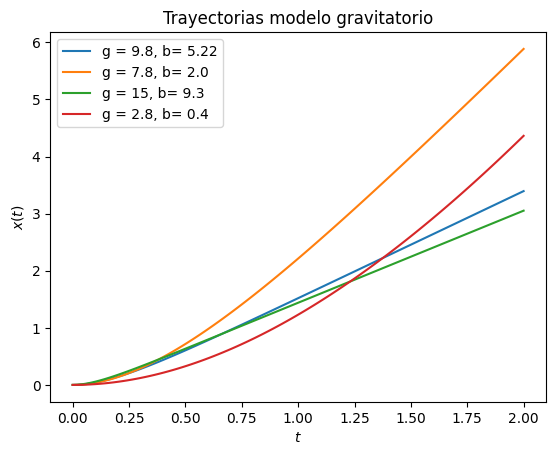
\includegraphics[width = 10 cm]{img/Trayectoria.png}
    \caption{Varias trayectorias con la dinámica gravitación sujeta a fricción para varias valores de los parámetros g,b.}
    \label{fig:trayectoria_gravedad}
\end{figure}

\subsection{Modelo Logístico}

Un modelo de crecimiento poblacional simple caracterizado por una ecuación diferencial es aquel que la tasa de cambio de la población es proporcional al tamaño actual de la población. Sea $P(t)$ el tamaño de la población al tiempo $t$. El modelo descrito es 
\begin{align}
    \frac{dP}{dt} = \lambda P(t)
    \label{3.1.20}
\end{align}
donde $\lambda$ es la tasa de crecimiento y con la condición $P(0) = P_0$. 

La solución explicita al modelo en (\ref{3.1.20}) es
\begin{align}
    P(t) = P_0 e^{\lambda t }
\end{align}
que es una función creciente en el tiempo. Sin embargo, este modelo solo es valioso para pequeños intervalos de tiempo, ya que el crecimiento en una la tasa de cambio de la población tiende a decaer a medida que se consumen los recursos. 

Para saldar con la dificultad planteada, podemos modelar la tasa de crecimiento de una población considerando tanto al tamaño de la población como a los recursos aún presentes. Consideremos a $K$ como la capacidad de sustento, que se puede interpretar como la cantidad máxima de población que los actuales recursos permiten mantener, entonces esperamos que a medida que crece la población, la tasa de crecimiento de la misma decresca.

El modelo que se propone es conocido como el modelo de crecimiento logístico. Este nos dice que el cambio de la población es proporcional al tamaño de la población misma así como a la proporción de recursos disponibles. Dicho modelo se puede escribir con la ecuación de Verhulst 
\begin{align}
    \frac{dP}{dt} = rP\left(1- \frac{P}{K}  \right)
\end{align}
donde $r$ es la tasa de crecimiento y $K$ la capacidad de sustento.

A pesar de que la ecuación diferencial del modelo de crecimiento logístico es no lineal tiene solución explicita. Notemos que la EDO pertenece a la familia de las EDO de Bernoulli, esto es tiene la forma
\begin{align*}
    \frac{dy}{dt} + P(x) y =Q(x) y^n
\end{align*}
y además puede transformar a una EDO lineal de primer orden con $u(x) = y ^{1-n}$.

Por tanto, del cambio $u(t) = P^{-1}$ obtenemos la solución explicita a (\ref{3.1.20})
\begin{align}
    P(t) = \frac{KP_0 e^{rt}}{K + P_0 \left(e^{rt}-1\right)}    
\end{align}
donde verificamos que $\lim_{t \rightarrow \infty} = K $. 

Podemos ver en la Fig \ref{fig:trayectoria_logistico} que sus trayectorias son no decrecientes y tiene asíntoticamente al parámetro $K$.


\begin{figure}
    \centering
    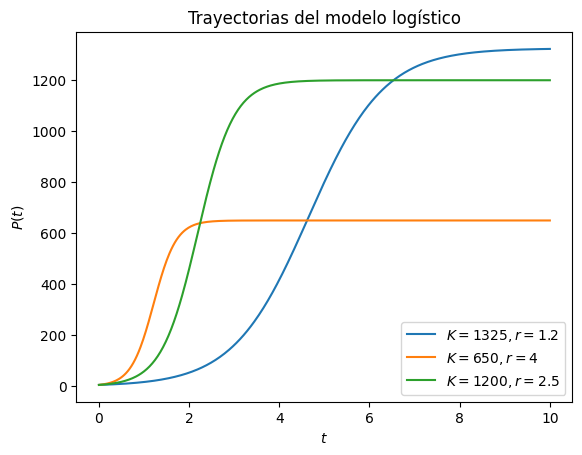
\includegraphics[width = 10 cm]{img/trayectoria_log.png}
    \caption{Varias trayectorias con la dinámica de crecimiento logístico para varias valores de los parámetros K,r.}
    \label{fig:trayectoria_logistico}
\end{figure}



\subsection{Modelo SIR}

Los modelos epidemiológicos clasifican a la población en clases que distinguen si han tenido o no cierta enfermedad. Un modelo que captura con buena aproximación a varias enfermedades se es el modelo SIR. Este propone dividir a las $N$ personas de una población en tres grupos:
\begin{enumerate}
    \item Susceptible ($S$): Todas las personas que no han tenido la enfermedad ni están enfermas del brote de interés.
    \item Infectado ($I$): Son las personas que actualmente portan el patógeno y son además un vector de transmisión.
    \item Recuperado ($R$): Para aquellas personas que se han recuperado de la enfermedad y ya tienen inmunidad o también para aquellas que perecieron.
\end{enumerate}

Así, el modelo propuesto supone que la tasa de cambios de las personas susceptibles decrece proporcionalmente a la cantidad de infectados y la cantidad de susceptibles restantes. De igual forma, la cantidad de recuperados crece con una tasa proporcional a la cantidad de infectados. La dinámica del modelo SIR se da con el siguiente sistema de EDO's
\begin{align}
    \frac{dS}{dt} &= -\beta S I \nonumber \\
    \frac{dI}{dt} &= \beta S I - \gamma I\\
    \frac{dR}{dt} &= \gamma I \nonumber
\end{align}
donde $\beta$ es la tasa de infección, $\gamma$ es la tasa de recuperación y $S + I + R = N$.

La solución explicita para $S(t), I(t), R(t)$ no existe en general, por ello se requieren métodos numéricos para resolver numéricamente para cada grupo y poder construir el forward map. En la Fig. \ref{fig:trayectoria_SIR} tenemos un ejemplo para un caso del modelo SIR con tasa de infección $\beta = 0.009$ y tasa de recuperación $\gamma = 0.5$


\begin{figure}
    \centering
    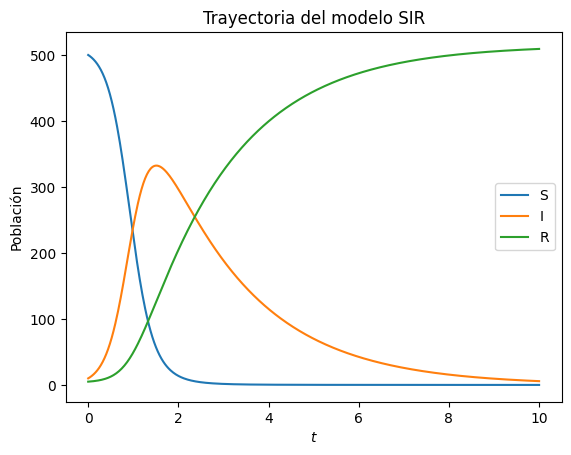
\includegraphics[width = 10 cm]{img/trayectoria_SIR.png}
    \caption{Trayectoria de cada grupo del modelo SIR con $\beta = 0.009$ y $\gamma = 0.5$.}
    \label{fig:trayectoria_SIR}
\end{figure}




% \section{Inferencia sin aproximación}
\section{Enfoque bayesiano al problema inverso}

Una vez establecidos los modelos sobre los que trabajaremos, nos enfocamos en abordar el problema inverso para los mismos. Para ello, es necesario tener a disposición una muestra de la trayectoria del modelo al cual deseamos inferir sus parámetros.

Según sea el caso, podemos tomar mediciones de caída de un objeto para ciertos tiempo, o podemos contar la población para cada intervalo de tiempo, observar los grupos de personas en un brote de cierto patógeno. Denotemos estas observaciones por $y_1, y_2, \cdots, y_n$. 

Sin embargo, no es fácil tener acceso a dicha muestra, por lo que optaremos por simular los datos directamente del modelo seleccionando los parámetros convenientemente y además agregar un ruido gaussiano. Es decir, tomamos $\theta$ fijo, luego consideramos los tiempos a los cuales corresponderá la muestra, denotados por $t_1, t_2, \cdots, t_n$. Posteriormente, con el forward map $F_{\theta}$ generado según el modelo (ya sea analítico o numérico) evaluamos para cada tiempo (denotado por $F_{\theta}(t_i)$) y agregamos un ruido $\varepsilon_i \sim N(0,\sigma^2)$. Así la muestra considerada se constituye por
\begin{align}
    y_i = F_{\theta}(t_i) + \varepsilon_i %\:\:\:\: \text{para } i = 1,2,\cdots,n.
\end{align}
para $i = 1,2, \cdots, n$. 

Una vez establecida la muestra $y_i$, ahora nuestro propósito es abordar el problema inverso, esto es buscamos $\theta$ tal que $y_i \approx F_{\theta}(t_i)$. Del capitulo 2 sabemos que hay varias maneras de abordar el problema, en adelante solamente se usará el enfoque bayesiano del problema inverso.

% \subsection{Distribución posterior}

\subsection{Forward map}
\subsection{Simulación con MCMC}
\subsection{Resultados}

\section{Inferencia con aproximación.}

\subsection{Regla de interpolación(aproximación de forward map)}
\subsection{Simulación MCMC}
\subsection{Resultados}

\newpage

\subsection{Experimentación con la convergencia.}

En esta sección se abordan las diferentes simulaciones para cada modelo. Empezando por el modelo de gravedad sujeto a fricción, nos interesa la distribución posterior de los parámetros $g$ y $b$. Con la metodología establecida y usando MCMC con la a priori \textcolor{red}{Grafico de la priori} anteriormente mencionada obtenemos una simulación de la distribución posterior conjunta. Tomando la marginal de cada parámetro y haciendo el histograma para la estimación de la distribución marginal tenemos las siguientes distribuciones posteriores marginales.


\textcolor{red}{Poner la distribución posterior marginal con Forward ordinario}

Consideremos ahora la distribución posterior conjunta obtenida con el Forward map aproximado. En este caso, se hace el experimento para la cantidad de 5,8,16 vecinos cercanos y a su vez cada uno de ello haciendo la malla cada vez más fina. Para cada Forward con la cantidad dada de vecinos cercanos se propone una malla en el espacio de parámetros $(g,b)\in \Theta$ de tamaño 10x10, 15x15, 30x30, 50x50.

La muestra inicial de la trayectoria que sigue el modelo se hace mediante simulación desde la misma ecuación diferencial dada por el modelo. Es de nuestra elección la cantidad de muestra $n$ que queremos para la distribución posterior conjunta de los parámetros. Sin embargo, para dicha simulación es necesario fijar dos parámetros, que llamaremos parámetros verdadero y obtener la trayectoria $x_t|\theta$. 

Para la simulación de los datos consideramos una muestra de 30 datos del modelo de gravedad en el intervalo de tiempo $[0,1.5]$. 

Las distribuciones posteriores marginales de $g$ se muestran en las figuras \ref{fig:g_01} \ref{fig:g_02}    \ref{fig:g_03} 

% \begin{figure}
%     \centering
%     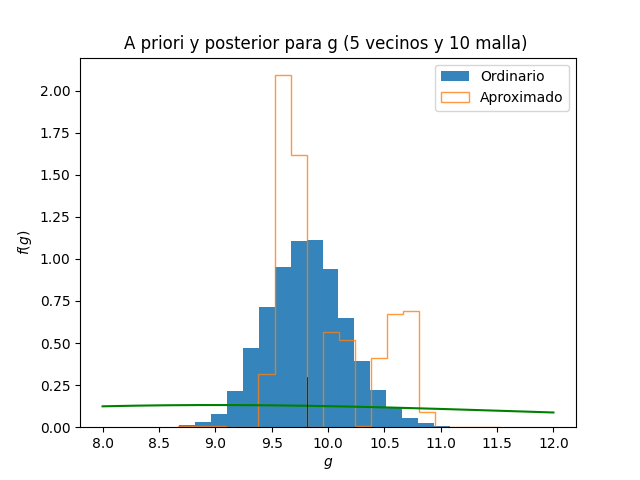
\includegraphics{img/posterior_g_1.png}
%     \caption{Caption}
%     \label{fig:enter-label}
% \end{figure}


% \begin{figure}
% \begin{subfigure}{.5\textwidth}
%   \centering
%   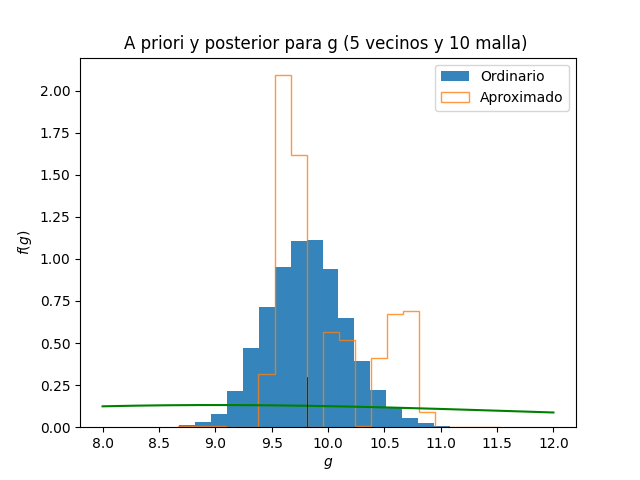
\includegraphics[width=.8\linewidth]{img/posterior_g_1.png}
%   \caption{1}
%   \label{fig:sfig2}
% \end{subfigure}
% \begin{subfigure}{.5\textwidth}
%   \centering
%   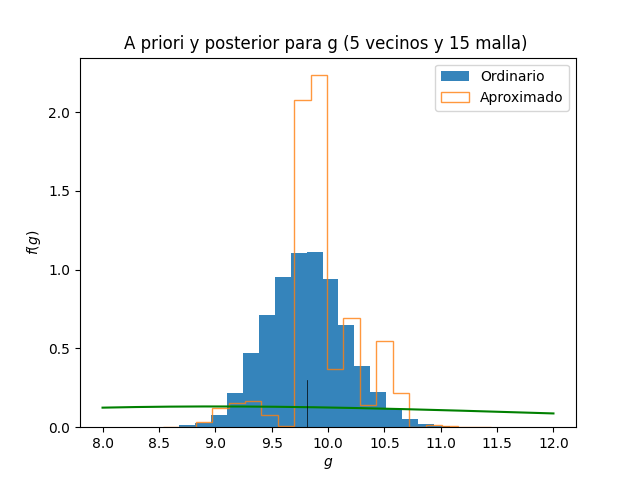
\includegraphics[width=.8\linewidth]{img/posterior_g_2.png}
%   \caption{2}
%   \label{fig:sfig1}
% \end{subfigure}%
% \begin{subfigure}{.5\textwidth}
%   \centering
%   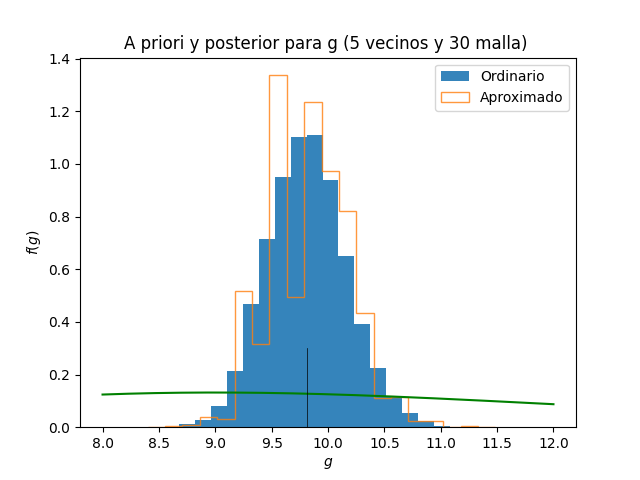
\includegraphics[width=.8\linewidth]{img/posterior_g_3.png}
%   \caption{3}
%   \label{fig:sfig2}
% \end{subfigure}
% \begin{subfigure}{.5\textwidth}
%   \centering
%   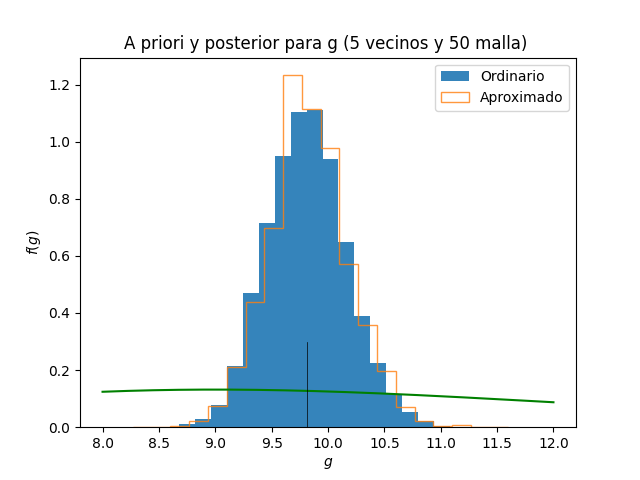
\includegraphics[width=.8\linewidth]{img/posterior_g_4.png}
%   \caption{4}
%   \label{fig:sfig2}
% \end{subfigure}
% \caption{plots of....}
% \label{fig:fig}
% \end{figure}

% 5 vecinos
\begin{figure}[h]
    \centering
    \subfloat[Subfigure 1 list of figures text][Posterior con Forward aproximado en malla de 10x10]{
    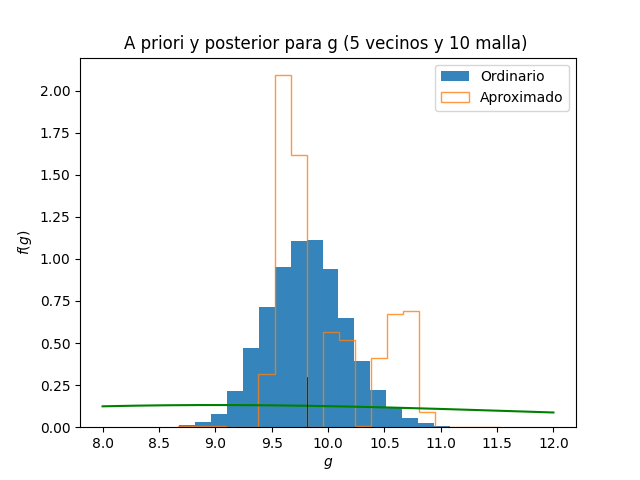
\includegraphics[width=0.4\textwidth]{img/posterior_g_1.png}
    \label{fig:subfig1}}
    \qquad
    \subfloat[Subfigure 2 list of figures text][Posterior con Forward aproximado en malla de 15x15]{
    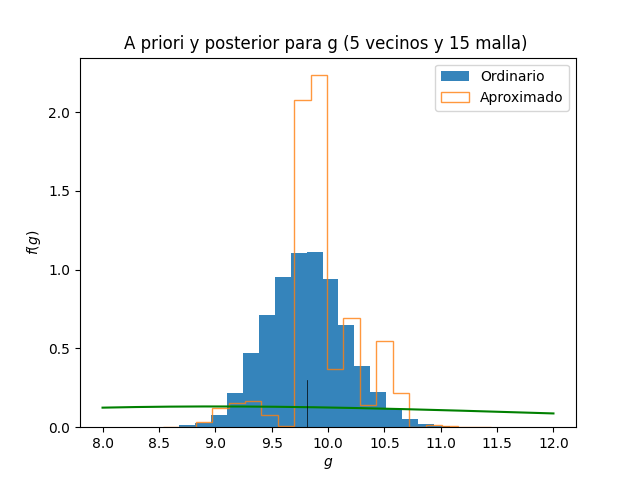
\includegraphics[width=0.4\textwidth]{img/posterior_g_2.png}
    \label{fig:subfig2}}
    \subfloat[Subfigure 3 list of figures text][Posterior con Forward aproximado en malla de 30x30]{
    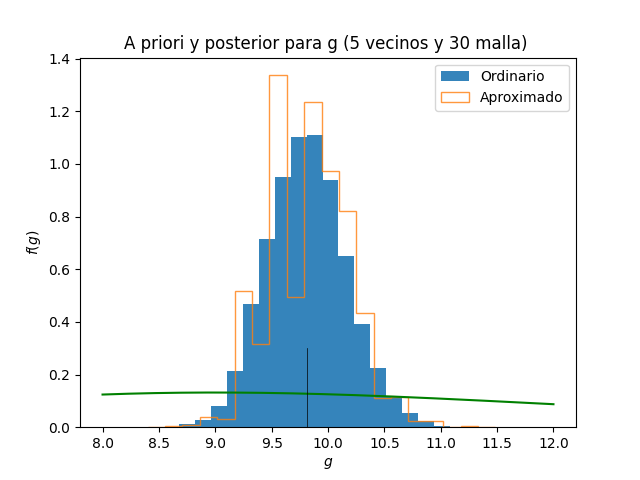
\includegraphics[width=0.4\textwidth]{img/posterior_g_3.png}
    \label{fig:subfig3}}
    \qquad
    \subfloat[Subfigure 4 list of figures text][Posterior con Forward aproximado en malla de 50x50]{
    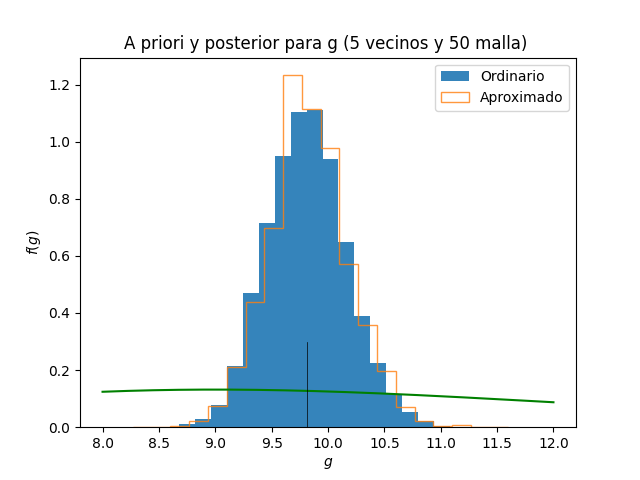
\includegraphics[width=0.4\textwidth]{img/posterior_g_4.png}
    \label{fig:subfig4}}
    \caption{Distribución posterior para $g$ con Forward ordinario y Forward aproximado con 5 vecinos cercanos.}
    \label{fig:g_01}
\end{figure}


% 8 vecinos
\begin{figure}[h]
    \centering
    \subfloat[Subfigure 1 list of figures text][Posterior con Forward aproximado en malla de 10x10]{
    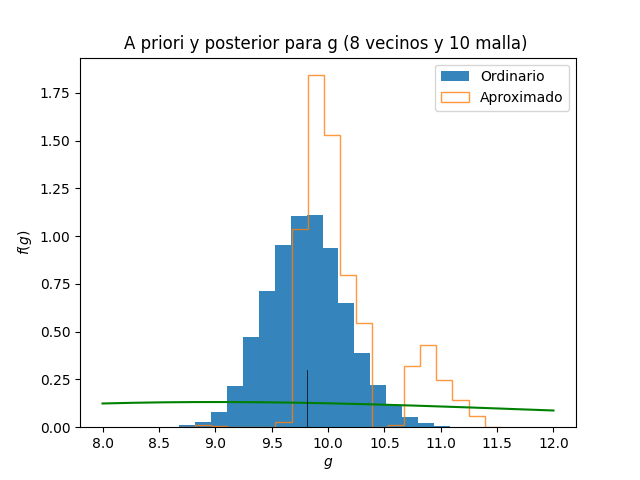
\includegraphics[width=0.4\textwidth]{img/posterior_g_5.png}
    \label{fig:subfig1}}
    \qquad
    \subfloat[Subfigure 2 list of figures text][Posterior con Forward aproximado en malla de 15x15]{
    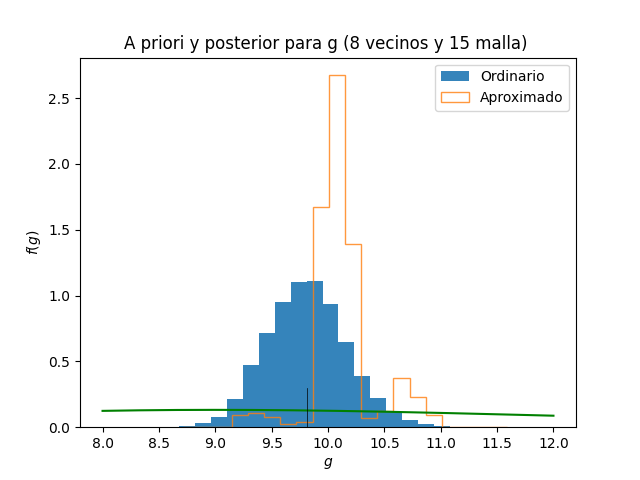
\includegraphics[width=0.4\textwidth]{img/posterior_g_6.png}
    \label{fig:subfig2}}
    \subfloat[Subfigure 3 list of figures text][Posterior con Forward aproximado en malla de 30x30]{
    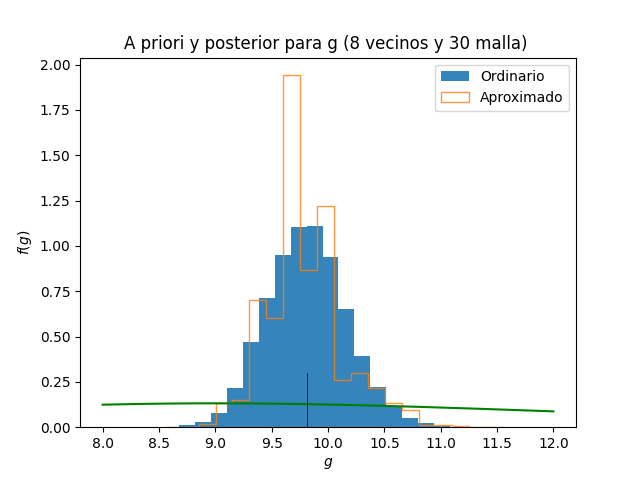
\includegraphics[width=0.4\textwidth]{img/posterior_g_7.png}
    \label{fig:subfig3}}
    \qquad
    \subfloat[Subfigure 4 list of figures text][Posterior con Forward aproximado en malla de 50x50]{
    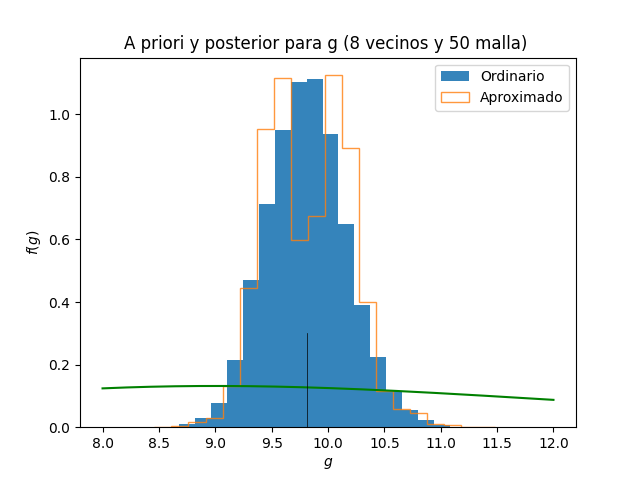
\includegraphics[width=0.4\textwidth]{img/posterior_g_8.png}
    \label{fig:subfig4}}
    \caption{Distribución posterior para $g$ con Forward ordinario y Forward aproximado con 8 vecinos cercanos.}
    \label{fig:g_02}
\end{figure}


% 16 vecinos
\begin{figure}[h]
    \centering
    \subfloat[Subfigure 1 list of figures text][Posterior con Forward aproximado en malla de 10x10]{
    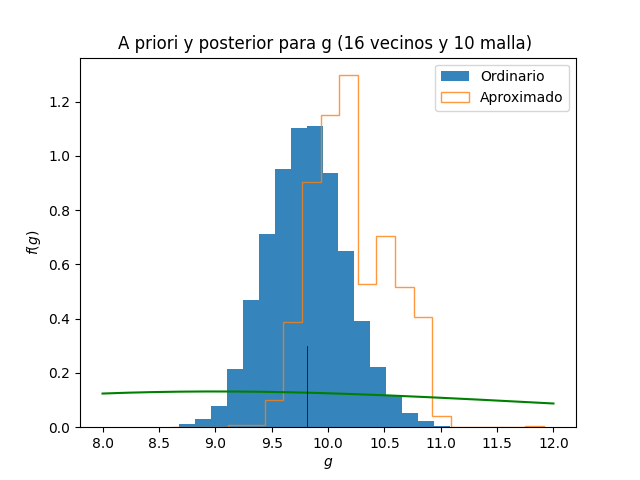
\includegraphics[width=0.4\textwidth]{img/posterior_g_9.png}
    \label{fig:subfig1}}
    \qquad
    \subfloat[Subfigure 2 list of figures text][Posterior con Forward aproximado en malla de 15x15]{
    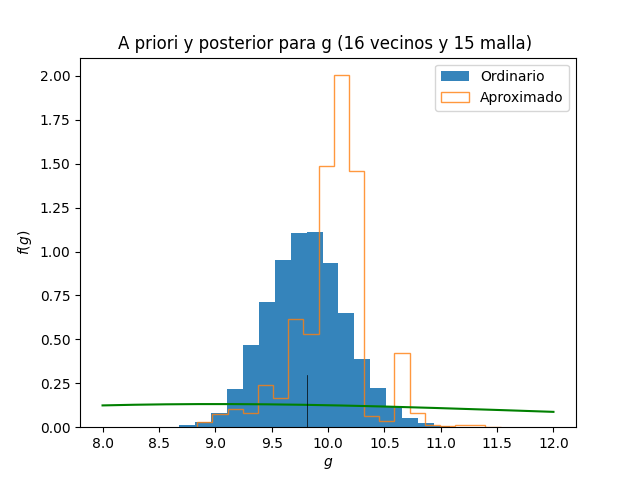
\includegraphics[width=0.4\textwidth]{img/posterior_g_10.png}
    \label{fig:subfig2}}
    \subfloat[Subfigure 3 list of figures text][Posterior con Forward aproximado en malla de 30x30]{
    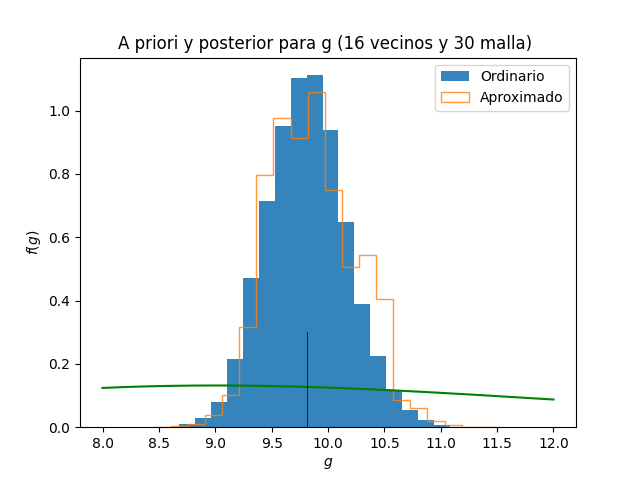
\includegraphics[width=0.4\textwidth]{img/posterior_g_11.png}
    \label{fig:subfig3}}
    \qquad
    \subfloat[Subfigure 4 list of figures text][Posterior con Forward aproximado en malla de 50x50]{
    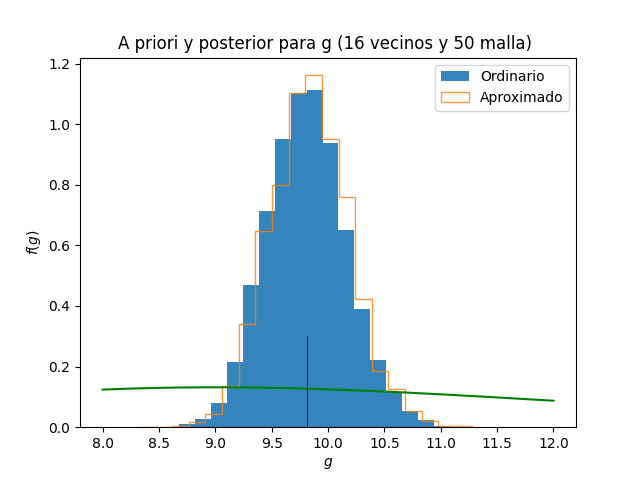
\includegraphics[width=0.4\textwidth]{img/posterior_g_12.png}
    \label{fig:subfig4}}
    \caption{Distribución posterior para $g$ con Forward ordinario y Forward aproximado con 16 vecinos cercanos.}
    \label{fig:g_03}
\end{figure}



Para el otro parámetro $b$ tenemos las siguientes posteriores

% 5 vecinos
\begin{figure}[h]
    \centering
    \subfloat[Subfigure 1 list of figures text][Posterior con Forward aproximado en malla de 10x10]{
    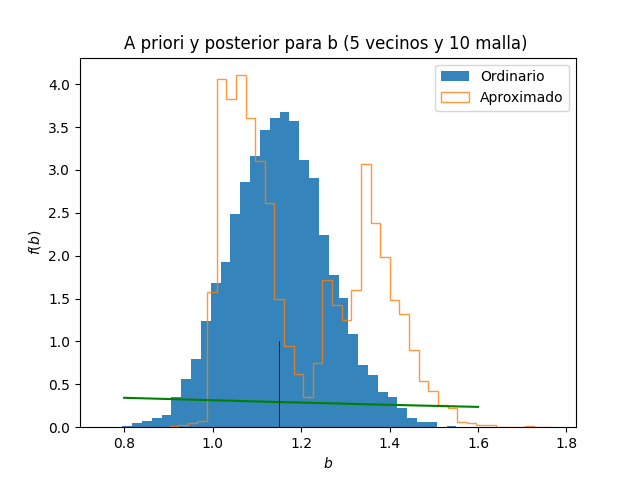
\includegraphics[width=0.4\textwidth]{img/posterior_b_1.png}
    \label{fig:subfig1}}
    \qquad
    \subfloat[Subfigure 2 list of figures text][Posterior con Forward aproximado en malla de 15x15]{
    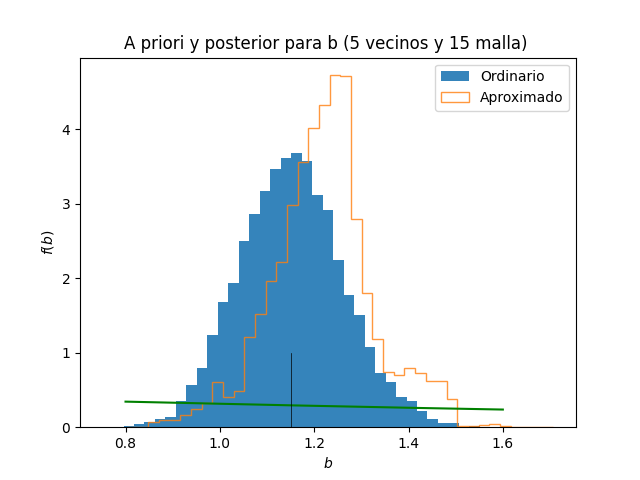
\includegraphics[width=0.4\textwidth]{img/posterior_b_2.png}
    \label{fig:subfig2}}
    \subfloat[Subfigure 3 list of figures text][Posterior con Forward aproximado en malla de 30x30]{
    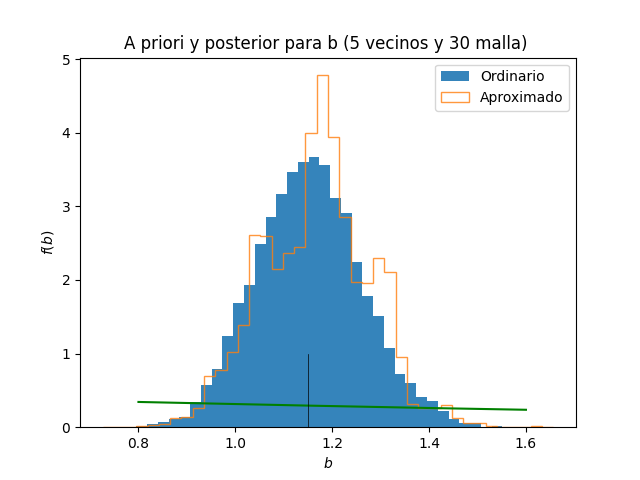
\includegraphics[width=0.4\textwidth]{img/posterior_b_3.png}
    \label{fig:subfig3}}
    \qquad
    \subfloat[Subfigure 4 list of figures text][Posterior con Forward aproximado en malla de 50x50]{
    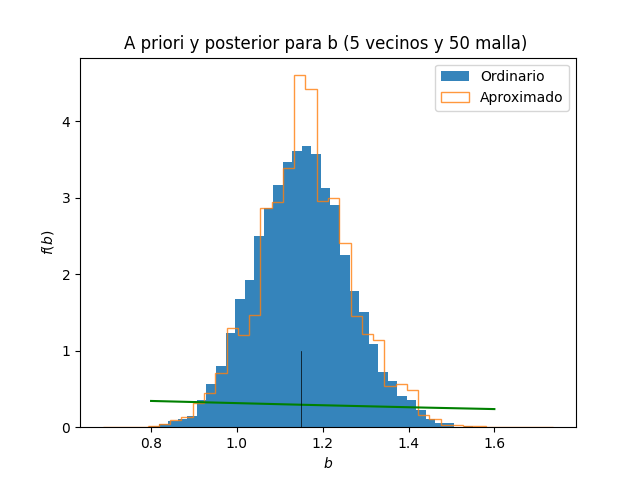
\includegraphics[width=0.4\textwidth]{img/posterior_b_4.png}
    \label{fig:subfig4}}
    \caption{Distribución posterior para $b$ con Forward ordinario y Forward aproximado con 5 vecinos cercanos.}
    \label{fig:g_04}
\end{figure}


% 8 vecinos
\begin{figure}[h]
    \centering
    \subfloat[Subfigure 1 list of figures text][Posterior con Forward aproximado en malla de 10x10]{
    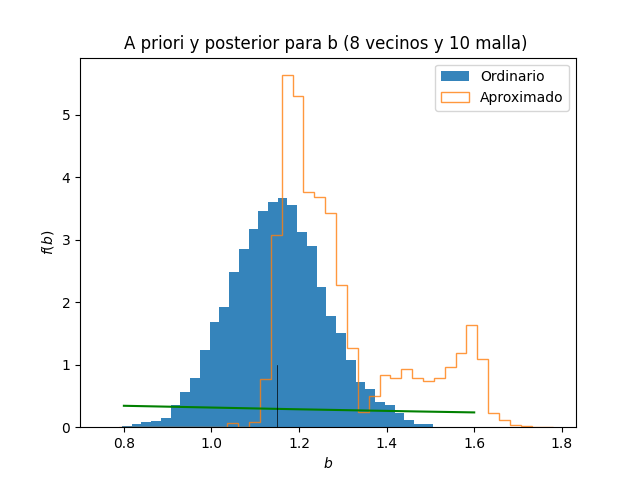
\includegraphics[width=0.4\textwidth]{img/posterior_b_5.png}
    \label{fig:subfig1}}
    \qquad
    \subfloat[Subfigure 2 list of figures text][Posterior con Forward aproximado en malla de 15x15]{
    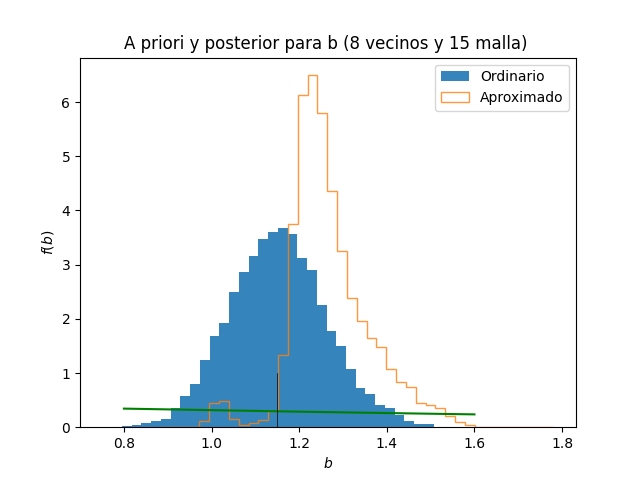
\includegraphics[width=0.4\textwidth]{img/posterior_b_6.png}
    \label{fig:subfig2}}
    \subfloat[Subfigure 3 list of figures text][Posterior con Forward aproximado en malla de 30x30]{
    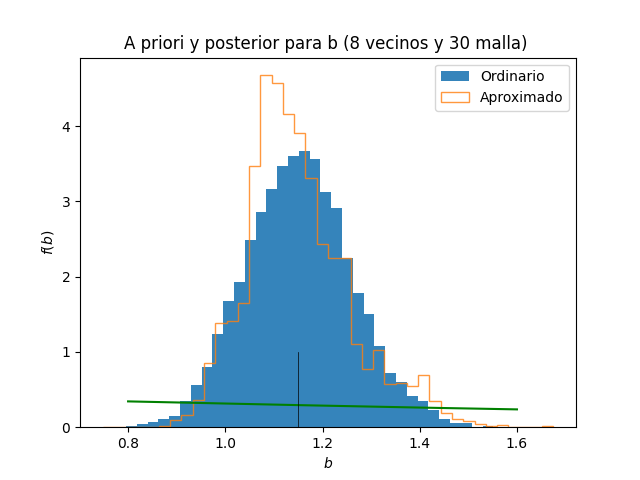
\includegraphics[width=0.4\textwidth]{img/posterior_b_7.png}
    \label{fig:subfig3}}
    \qquad
    \subfloat[Subfigure 4 list of figures text][Posterior con Forward aproximado en malla de 50x50]{
    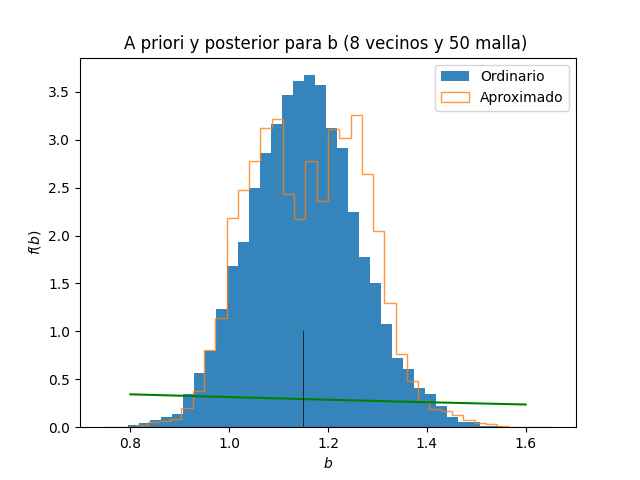
\includegraphics[width=0.4\textwidth]{img/posterior_b_8.png}
    \label{fig:subfig4}}
    \caption{Distribución posterior para $b$ con Forward ordinario y Forward aproximado con 8 vecinos cercanos.}
    \label{fig:g_05}
\end{figure}



% 16 vecinos
\begin{figure}[h]
    \centering
    \subfloat[Subfigure 1 list of figures text][Posterior con Forward aproximado en malla de 10x10]{
    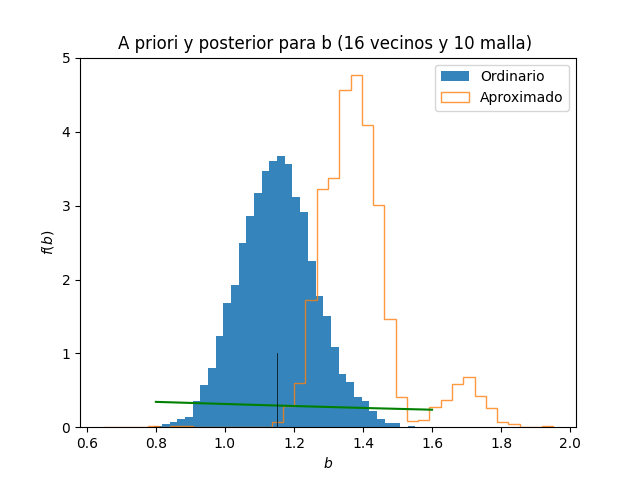
\includegraphics[width=0.4\textwidth]{img/posterior_b_9.png}
    \label{fig:subfig1}}
    \qquad
    \subfloat[Subfigure 2 list of figures text][Posterior con Forward aproximado en malla de 15x15]{
    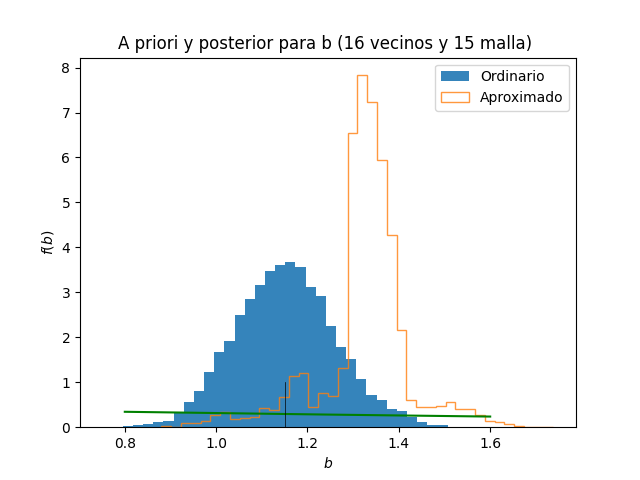
\includegraphics[width=0.4\textwidth]{img/posterior_b_10.png}
    \label{fig:subfig2}}
    \subfloat[Subfigure 3 list of figures text][Posterior con Forward aproximado en malla de 30x30]{
    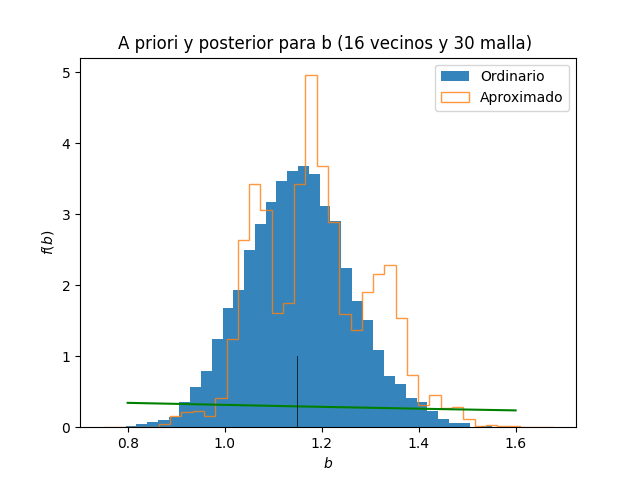
\includegraphics[width=0.4\textwidth]{img/posterior_b_11.png}
    \label{fig:subfig3}}
    \qquad
    \subfloat[Subfigure 4 list of figures text][Posterior con Forward aproximado en malla de 50x50]{
    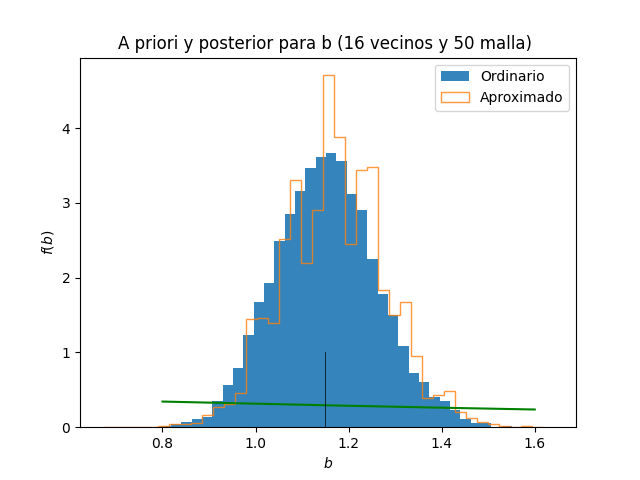
\includegraphics[width=0.4\textwidth]{img/posterior_b_12.png}
    \label{fig:subfig4}}
    \caption{Distribución posterior para $b$ con Forward ordinario y Forward aproximado con 16 vecinos cercanos.}
    \label{fig:g_06}
\end{figure}
